% GENERATED by build_tex.py (preprint: real commit hashes)
\section{Supplementary figures}\label{app:supp}


\begin{figure}[h]
  \centering
  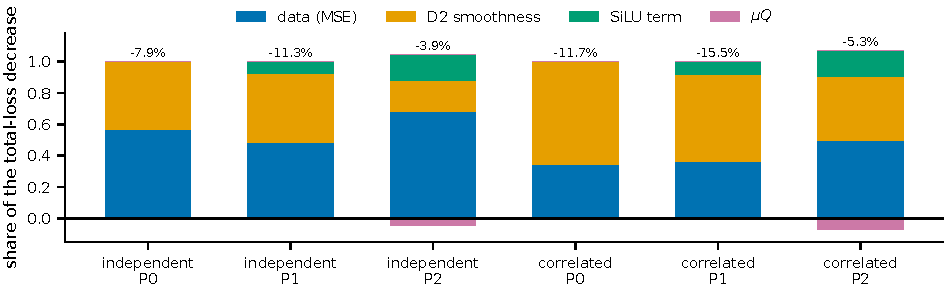
\includegraphics[width=\linewidth]{figS1_lossdecomp.pdf}
  % CAPTION-DRAFT: review (numbers from paper2/figures/figS1_lossdecomp.json)
  \caption{Post hoc loss decomposition (synthetic, early$\to$polished): share of the total-loss decrease from each term, pooled over the 8 seeds of each cell. independent P0: data 0.57, D2 0.43 (median total change -7.9\%); independent P1: data 0.49, D2 0.44 (median total change -11.3\%); independent P2: data 0.68, D2 0.20 (median total change -3.9\%); correlated P0: data 0.35, D2 0.65 (median total change -11.7\%); correlated P1: data 0.37, D2 0.55 (median total change -15.5\%); correlated P2: data 0.50, D2 0.40 (median total change -5.3\%).}
  \label{fig:S1}
\end{figure}


\begin{figure}[h]
  \centering
  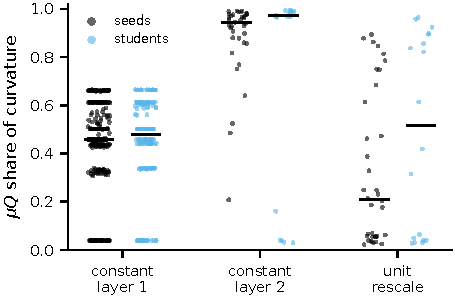
\includegraphics[width=0.5\linewidth]{figS2_gaugecheck.pdf}
  % CAPTION-DRAFT: review (numbers from paper2/figures/figS2_gaugecheck.json)
  \caption{Post hoc gauge check at the $\mu = 10^{-4}$ certified minima: share of the curvature along each least-squares gauge direction contributed by $\mu Q$. Medians: constant shift in layer 1, real-data seeds 0.46 ($n = 288$); constant shift in layer 1, students (trained on a frozen teacher) 0.48 ($n = 144$); constant shift in layer 2, real-data seeds 0.94 ($n = 36$); constant shift in layer 2, students 0.97 ($n = 18$); unit rescaling, real-data seeds 0.21 ($n = 36$); unit rescaling, students 0.52 ($n = 18$).}
  \label{fig:S2}
\end{figure}


\begin{figure}[h]
  \centering
  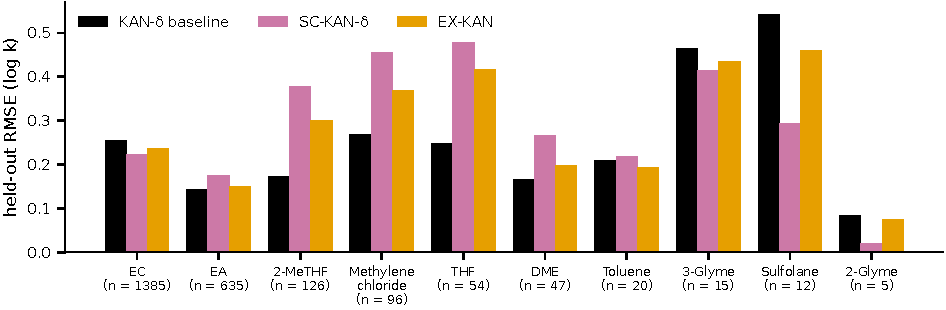
\includegraphics[width=\linewidth]{figS3_loco.pdf}
  % CAPTION-DRAFT: review (numbers from paper2/figures/figS3_loco.json)
  \caption{Leave-one-co-solvent-out RMSE per fold (5-seed ensembles, early state) for the KAN-$\delta$ baseline, SC-KAN-$\delta$ and EX-KAN. Unweighted means: KAN-$\delta$ baseline 0.2554; SC-KAN-$\delta$ 0.2923; EX-KAN 0.2834. The EA fold uses the fold A rows.}
  \label{fig:S3}
\end{figure}
